%%%%%%%%%%%%%%%%%%%%%%%%%%%
% CHAPTER 6 -- MAIN STUDY
%%%%%%%%%%%%%%%%%%%%%%%%%%%
%%%%%%%%%%%%%%%%%%%%%%%%%%%%%%%%%%%%%%%%%%%%%%%%%%%%%%%%%%%%%%%%%%%%%%%%%%%%%%%%%%%%%%%%%%
% Richard Boardman PhD Thesis: Improving Tool Support for Personal Information Management
%%%%%%%%%%%%%%%%%%%%%%%%%%%%%%%%%%%%%%%%%%%%%%%%%%%%%%%%%%%%%%%%%%%%%%%%%%%%%%%%%%%%%%%%%%

\textbf{Chapter notes}:
%%%%%%%%%%%%%%%%%%%%%%%
\begin{itemize}
	\item \textit{THINK: Relate to overall PhD aims}
	\item THINK: Data and discussion here appear to raise potential conflicts with earlier findings - need to think carefully about how to frame them (Angela: \textit{"`OK to admit that you learned something"'}
	\item THINK: how to present study?
	\begin{enumerate}
		\item Further study, investigate further in follow-up to previous study
		\item Evaluation of WorkspaceMirror
		\item Evaluation as theory-building
	\end{enumerate}
	\item \textit{THINK: how to separate results and discussion in this chapter}
	\item \textit{THINK: how to separate this chapter and the next}
\end{itemize}

%%%%%%%%%%%%%%%%%%%%%%%%%%%%%%%%%%%%%%%%
%%%%%%%%%%%%%%%%%%%%%%%%%%%%%%%%%%%%%%%%
\section{Introduction}
\label{main-study:introduction}
%%%%%%%%%%%%%%%%%%%%%%%%%%%%%%%%%%%%%%%%
%%%%%%%%%%%%%%%%%%%%%%%%%%%%%%%%%%%%%%%%

%%%%%%%%%%%%%%%
% LEAD-IN INTRO
% include link to previous chapters
%%%%%%%%%%%%%%%
This section describes a field-study based evaluation of the WM prototype described in  \textbf{Chapter~\ref{chapter:design}}\footnote{\textit{This draft of Chapter 6 MAIN STUDY was printed \today.}}.

% Relate to overall methodology (DIAGRAM to illustrate?}

%%%%%%%%%%%%%%%%%%%%%%%%%%%%%%%%
% Overview of the chapter}
%%%%%%%%%%%%%%%%%%%%%%%%%%%%%%%%
The chapter is structured as follows.  First, \textbf{Section~\ref{main-study:aims}} outlines the study objectives.


\textbf{Set out contributions of this chapter towards overall thesis}:
%%%%%%%%%%%%%%%%%%%%%%%%%%%%%%%%%%%%%%%%%%%%%%%%%%%%%%%%%%%%%%%%%%%%%%\begin{itemize}
\begin{itemize}
	\item 
\end{itemize}



%%%%%%%%%%%%%%%%%%%%%%%%%%%%%%%%%%%%%%%%
%%%%%%%%%%%%%%%%%%%%%%%%%%%%%%%%%%%%%%%%
\section{Aims}
\label{main-study:aims}
%%%%%%%%%%%%%%%%%%%%%%%%%%%%%%%%%%%%%%%%
%%%%%%%%%%%%%%%%%%%%%%%%%%%%%%%%%%%%%%%%

\textbf{What is evaluation? Why evaluate?}:
%%%%%%%%%%%%%%%%%%%%%%%%%%%%%%%%%%%%%%%%%%%
\begin{itemize}
	\item Definition (Robson: attempt to assess worth of some innovation or intervention)
	\item Choice of method. See below (SP)
\end{itemize}
	
\textbf{General Aims}:
%%%%%%%%%%%%%%%%%%%%%%	
\begin{itemize}
	\item Need for evaluation of WorkspaceMirror - standard component of HCI practice, but also:
	\item Ethnographic perspective: chance for more study, and:
	\item Design Science perspective, Artifact as theory-nexus. Evaluation as theory-building/validation.
\end{itemize}


\textbf{Introduce idea of fieldwork as dual-purpose research vehicle}:
%%%%%%%%%%%%%%%%%%%%%%%%%%%%%%%%%%%%%%%%%%%%%%%%%%%%%%%%%%%%%%%%%%%%%%
\begin{itemize}
	\item This is actually opportunity for further study/investigation as well
	\item Therefore dual-purpose research vehicle
	\item Design-based research
	\item \textit{THINK: Base methodology -- combining study of work practice and design intervention~\cite{blomberg:96} -- but not cooperative prototyping.}
\end{itemize}


%%%%%%%%%%%%%%%%%%%%%%%%%%%%%%%%
\subsection{Aims of the Main Study}
%%%%%%%%%%%%%%%%%%%%%%%%%%%%%%%%
\begin{itemize}
	\item \textit{THINK: rationale for choice of aims}
	\item Empirical Aims -- a Dual-purpose Research Vehicle:
	%%%%%%%%%%%%%%%%%%%%%%%%%%%%%%%%%%%%%%%%%%%%%%%%%%%%%%%%
	\begin{itemize}
		\item Evaluate WorkspaceMirror. One focus equals (Formative) evaluation of WorkspaceMirror
		\item Use this evaluation as basis to explore potential for unification (pros and cons)
		\item \textit{THINK: talk about design intervention, and iteration}
		\item Provide context for further study into PIM behaviour - provide insights into PIM (analyze practice)
	\end{itemize}

	\item Methodological Aims:
	%%%%%%%%%%%%%%%%%%%%%%%%%%
	\begin{itemize}
		\item Operationalization/continued evelopment of Cross-tool Study/Evaluation Methodology
		\item Proof of practice/straw-man/test-case
		\item Exploratory nature due to lack of any evaluation approach, need to develop evaluation criteria - basis for further research
	\end{itemize}
	
\end{itemize}


%%%%%%%%%%%%%%%%%%%%%%%%%%%%%%%%%%%%%%%%%%%%%%%%%%%%%%%%%%%%%%
\subsection{Challenges of evaluating PIM tools (OVERLAP2)}
%%%%%%%%%%%%%%%%%%%%%%%%%%%%%%%%%%%%%%%%%%%%%%%%%%%%%%%%%%%%%%

\textbf{See Appendix}:
%%%%%%%%%%%%%%%%%%%%%%
\begin{itemize}
	\item Compounded challenges with this type of activity. Reasons why so rarely evaluated?
	\item Compounded again here as: 1 cross-tool feature leads to effects on multiple tools
	\item \textit{THINK: extract key points to expand here}
\end{itemize}



%%%%%%%%%%%%%%%%%%%%%%%%%%%%%%%%%%%%%%%%%
\subsection{Choice of evaluation methods}
%%%%%%%%%%%%C%%%%%%%%%%%%%%%%%%%%%%%%%%%%

\textbf{Overview of different evaluation methods}:
%%%%%%%%%%%%%%%%%%%%%%%%%%%%%%%%%%%%%%%%%%%%%%%%%%%%%%%%%%%%%%%%%%%
\begin{itemize}
	\item Each reflect philosophy and needs
	\item Choice: lab or contextualized/fieldwork
	\item Choice: short-term or longtitudinal
	\item THINK: get survey from textbook
\end{itemize}

\textbf{Choice of method and expand rationale behind decision}:
%%%%%%%%%%%%%%%%%%%%%%%%%%%%%%%%%%%%%%%%%%%%%%%%%%%%%%%%%%%%%%%%
\begin{itemize}
	\item textbf{Therefore choice of fieldwork-based evaluation}
	\item \textbf{Situated} (own data, naturalistic, contextualized) -- must be evaluated in work context (a la Suchman and co?). Critique of lab evals?
	\item \textbf{Long-term} (watch over time) -- desire to encompass both routine and exceptional events.
	\item \textbf{Cross-tool}
	\item \textbf{Exploratory} -- due to lack of previous work to build on
\end{itemize}


		

%%%%%%%%%%%%%%%%%%%%%%%%%%%%%%%%%%%%%%%%%%%%%%%%%%%%%
\subsection{Key Fieldwork-based Study/Evaluation Challenges}
%%%%%%%%%%%%%%%%%%%%%%%%%%%%%%%%%%%%%%%%%%%%%%%%%%%%%%

\textbf{Expected challenges inherent in fieldwork method}:
\begin{itemize}

	\item \textbf{Standard evaluation concerns}:
	%%%%%%%%%%%%%%%%%%%%%%%%%%%%%%%%%%%%%%%%%%%%%
	\begin{itemize}
		\item 	All the normal evaluation concerns (e.g. ecological validity)
	\end{itemize}

	\item \textbf{Problems due to fieldwork as choice of method}:
	%%%%%%%%%%%%%%%%%%%%%%%%%%%%%%%%%%%%%%%%%%%%%%%%%%%%%%%%%%%%%%%
	\begin{itemize}
		\item logistics: roll-out, install, support
		\item Time: usage in short/long-term. Benefits just appear in long-term?
	\end{itemize}

	\item \textbf{Problems due to evaluation of PIM tool (OVERLAP2)}:
	%%%%%%%%%%%%%%%%%%%%
	\begin{itemize}
		\item Ethical issues of working with personal data
		\item individual differences
		\item Time: usage in short/long-term. Benefits just appear in long-term?
	\end{itemize}
		
	\item \textbf{Problems due to cross-tool nature} -- evaluating a distributed PIM design:
	%%%%%%%%%%%%%%%%%%%%%%%%%%%%%%%%%%%%%%
	\begin{itemize}
		\item Tools: inter-dependencies between multiple tools
	\end{itemize}
		
\end{itemize}


%%%%%%%%%%%%%%%%%%%%%%%%%%%%%%%%%%%%%%%
\subsection{Setting scope of the study}
%%%%%%%%%%%%%%%%%%%%%%%%%%%%%%%%%%%%%%%

\textbf{Scoping Assumptions}:
%%%%%%%%%%%%%%%%%%%%%%%%%%%%%%%%%%%%%%%%%%%%%%%%%%%%%%%%%%%%%%%%%%%%%%%%%
\begin{itemize}
	\item Done to compensate for ambitious CROSS-TOOL scope, somewhat unrealistic but still more realistic than most
	\item One computer per participant
	\item Three tools per computer
	\item Document space - focus on one nominated area
	\item Personal as before
\end{itemize}
	
		








%%%%%%%%%%%%%%%%%%%%
%%%%%%%%%%%%%%%%%%%%
\section{Method}
\label{main-study:method}
%%%%%%%%%%%%%%%%%%%%
%%%%%%%%%%%%%%%%%%%%

Study process is illustrated in: \textbf{Figure~\ref{fig:main-study:method-overview}}:
\begin{enumerate}
	\item Prelims (e.g. disclosure agreement)
	\item Snapshot Profile Interview (PROFILE)
	\item Longitudinal Phase 1 - pre-install profiling (STUDY PHASE)
	\item Interim interview and installation of WorkspaceMirror.
	\item Longitudinal Phase 2 - extended field trial of WorkspaceMirror (EVALUATION PHASE)
	\item Closing interview
	\item \textit{THINK: can I talk about a quasi-experimental method? (REF: Robson)}
\end{enumerate}

%%%%%%%%%%%%%%%%%%%%%%%%%%%%%%%
\subsection{Selection of users}
%%%%%%%%%%%%%%%%%%%%%%%%%%%%%%%
\begin{itemize}
	\item Some from feasibility study
	\item Ethical/privacy issues
	\item Reasons for choosing colleagues: upsides and downsides. Consideration of other options. Acknowledge potential bias 
	\item Compare with Bellotti's difficulties, Whittaker. 
	\item Small number -- no chance of statistical significance
\end{itemize}

\subsection{Profiling Interview}
%%%%%%%%%%%%%%%%%%%%%%%%%%%%%%%%
\begin{itemize}
	\item \textit{THINK: need subsection for prelims before this?}
	\item Not told (toomuch) about nature of tool in advance
	\item Interview. Refer to experimental material in appendix (eg. q'aire)
	\item Questionnaire design?  See appendix.
	\item Time, location
\end{itemize}

\subsection{Phase 1: Profile and study}
%%%%%%%%%%%%%%%%%%%%%%%%%%%%%%%%%%%%%%%
\begin{itemize}
	\item Multiple methods of (hopefully complementary) data collection to reduce inappropriate certainty, and enhance interpretability.
	\item Data collection: diary and log/snapshots (WorkspaceSnapper tool to capture metadata)
	\item Refer to experimental material in appendix (eg. q'aire)
	\item Time
\end{itemize}

\subsection{Intervention: Installation of WorkspaceMirror}
%%%%%%%%%%%%%%%%%%%%%%%%%%%%%%%%%%%%%%%%%%%%%%%%%%%%%%%%%%
\begin{itemize}
	\item Design as an intervention in the study process
	\item Installation process and training, mini-interview, time
	\item Installation problems -- User by user list of issues, Windows compatibility issues
\end{itemize}

\subsection{Phase 2: Evaluation of WorkspaceMirror}
%%%%%%%%%%%%%%%%%%%%%%%%%%%%%%%%%%%%%%%%%%%%%%%%%%%
\begin{itemize}
	\item Data collection: diary and log/snapshots as before
	\item Occasionally had to sort problems
	\item Ended with closing interview
	\item Time
\end{itemize}

\section{Data Analysis and triangulation}
%%%%%%%%%%%%%%%%%%%%%%%%%%%%%%%%%%%%%%%%%%%%%%%%%%%


\textbf{Data Collection}
%%%%%%%%%%%%%%%%%%%%%%%%
\begin{itemize}
	\item Mass of data collected via the range of methods. Data overload!
	\item Attempted to
\end{itemize}

\textbf{Triangulation}:
%%%%%%%%%%%%%%%%%%%%%%%
\begin{itemize}
	\item Triangulation - collation of data from multiple methods (objective and subjective)
	\item Workspace Evolution Transcript (example(s))
\end{itemize}

\textbf{Analysis of data}
%%%%%%%%%%%%%%%%%%%%%%%%%%
\begin{itemize}
		\item Learning from lessons of previous studies?
		\item Coding scheme
		\item Coding of data. Identification of common themes and issues as they emerged. IRRT?
		\item Extraction of critical incidents, most frequent and important issues and problems
		\item Main themes analysed around
		\item Cross-comparison between tools for each user
		\item Cross-comparison between users for each tool
		\item \textit{ONGOING!!!}
\end{itemize}





%%%%%%%%%%%%%%%%%%%%%%%%%%%%%%%%%%%%%%
% %%%%%%%%%%%%%%%%%%%%%%%%%%%%%%%%%%%%
% FIGURE - Main Study Process Overview
% %%%%%%%%%%%%%%%%%%%%%%%%%%%%%%%%%%%%
%%%%%%%%%%%%%%%%%%%%%%%%%%%%%%%%%%%%%%
\begin{figure}[t]
	\begin{center}
		\leavevmode
		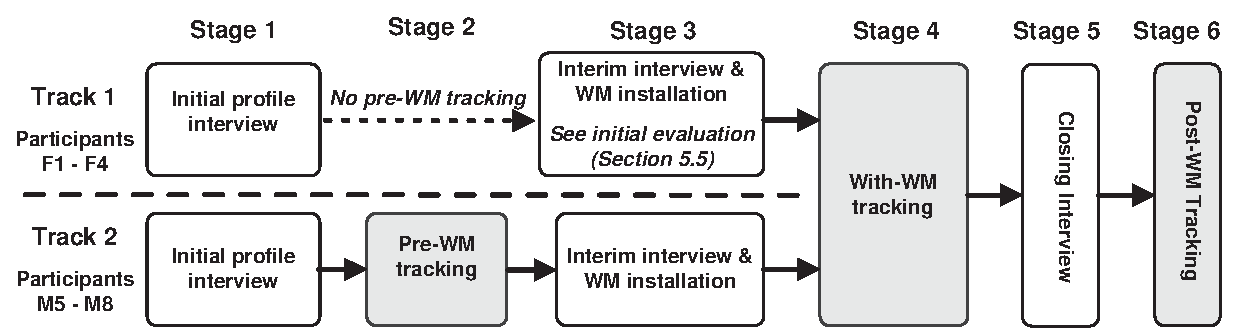
\includegraphics[height=2in, width=.9 \textwidth]{pictures/main-study/main-study-method.pdf}
	\end{center}
	\caption{Main Study: overview of method}
	\label{fig:main-study:method-overview}
\end{figure}



%%%%%%%%%%%%%%%%%%%%%%%%%%%%%%%
%%%%%%%%%%%%%%%%%%%%%%%%%%%%%%%
\section{Chapter Conclusion}
\label{main-study:chapter-summary}
%%%%%%%%%%%%%%%%%%%%%%%%%%%%%%%
%%%%%%%%%%%%%%%%%%%%%%%%%%%%%%%

\textbf{Retouch contributions}
%%%%%%%%%%%%%%%%%%%%%%%%%%%%%%

%%%%%%%%%%%%%%%%%%%%%%%%%%%%%%%%%%%%%%%%%%%%
\subsection{Moving on: Towards Deeper Insights}
%%%%%%%%%%%%%%%%%%%%%%%%%%%%%%%%%%%%%%%%%%%%

Set the scene for the discussion chapter, \textbf{Chapter~\ref{chapter:discussion}} ...

%%%%%%%%%%%%%%%%%%%%%%%%%%%%%%%%%%%%%%%%%%%%%%%%%%%

\textit{This draft of Chapter 6 MAIN STUDY was printed \today}
%%%%%%%%%%%%%%%%%%%%%%%%%%%%%%%%%
% FIN THESIS Chapter 6 MAIN STUDY
%%%%%%%%%%%%%%%%%%%%%%%%%%%%%%%%%



 


